\chapter{Bedienung des Benutzers}

Die Kalenderapp bietet dem Benutzer eine übersichtliche und benutzerfreundliche Bedienoberfläche, die es ermöglicht, Schulungsdaten effektiv zu verwalten und zu organisieren. 
Wenn man die App öffnet befindet man sich auf der Startseite \ref{Home}.  Hier befinden sich allgemeine Informationen über die App und weiter unten befindet sich ein Link zu Rechtlichem/ zum Impressum \ref{Imp}.
\begin{figure}[htbp!]
        \centering
        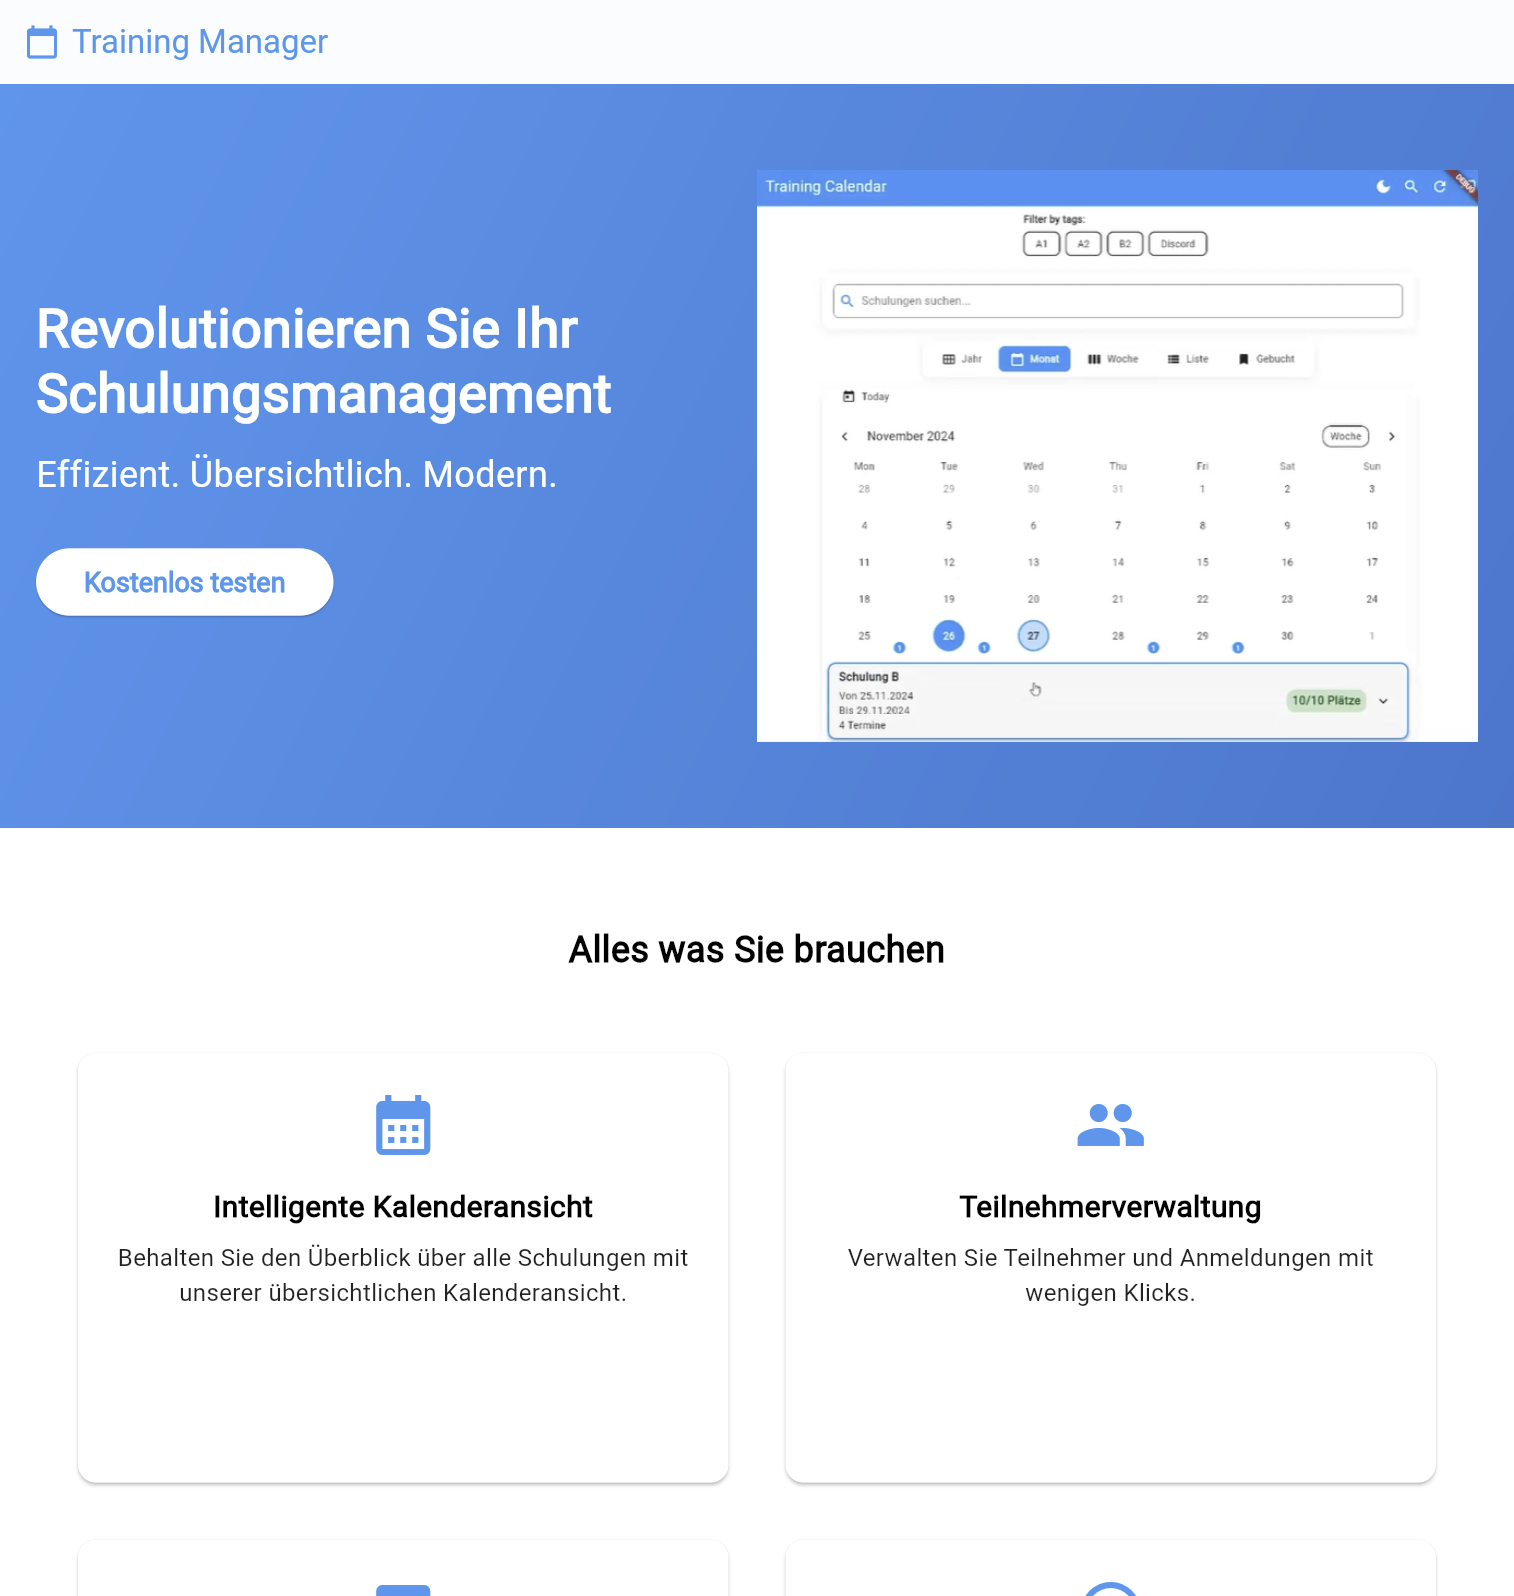
\includegraphics[scale=0.2]{img/flutter_31.png}
        \caption{Startseite}
        \label{Home}
    \end{figure}

\begin{figure}[htbp!]
        \centering
        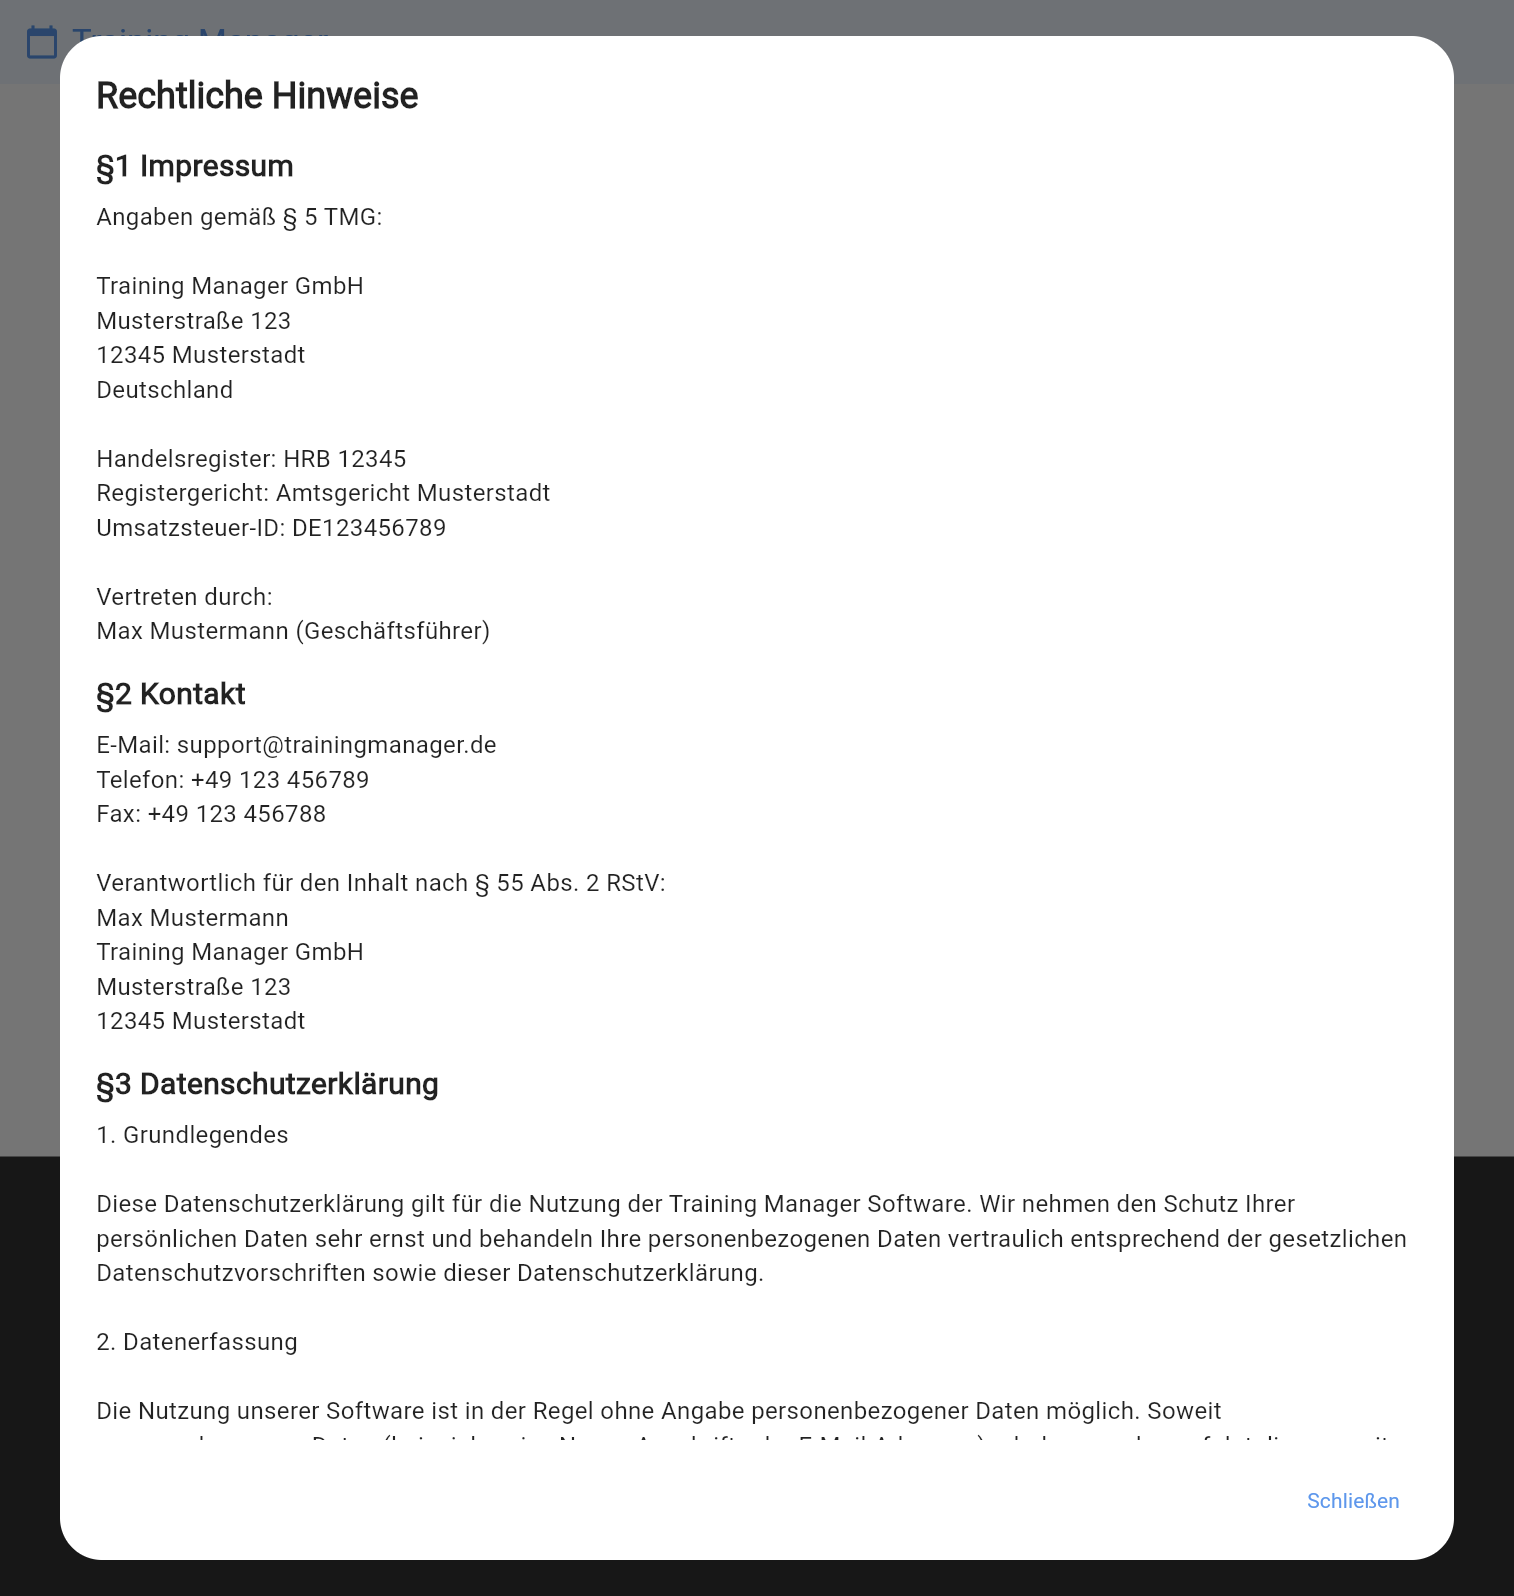
\includegraphics[scale=0.2]{img/flutter_32.png}
        \caption{Impressum}
        \label{Imp}
    \end{figure}
Mit dem Button “Kostenlos testen” gelangt man zum tatsächlichen Kalender.
Als Benutzer kann man oben in der Navigationsleiste zwischen verschiedenen Modi wechseln, wie Jahr, Monat, Woche, Liste und einer Buchungsübersicht, indem man auf die entsprechenden Buttons klickt. Standardmäßig gelangt man zur Monatsansicht.
Die App bietet eine intuitive Navigation, bei der der Benutzer zwischen den verschiedenen Ansichten hin und her wechseln kann. Alle Daten sind in einer klaren, strukturierten Form präsentiert, um eine effiziente Nutzung und eine schnelle Orientierung zu gewährleisten.
Details zu den verschiedenen Ansichten:
\begin{itemize}
    \item \textbf{Jahresansicht:} In dieser Ansicht (\ref{Jahr}) sieht der Benutzer das gesamte Jahr auf einen Blick. Alle Schulungsdaten sind übersichtlich auf dem Jahreskalender verzeichnet, sodass der Benutzer schnell einen Überblick über alle geplanten Schulungen und Termine erhält. Diese Ansicht eignet sich besonders, um langfristige Planungen und Übersichten zu erstellen.
\begin{figure}[htbp!]
        \centering
        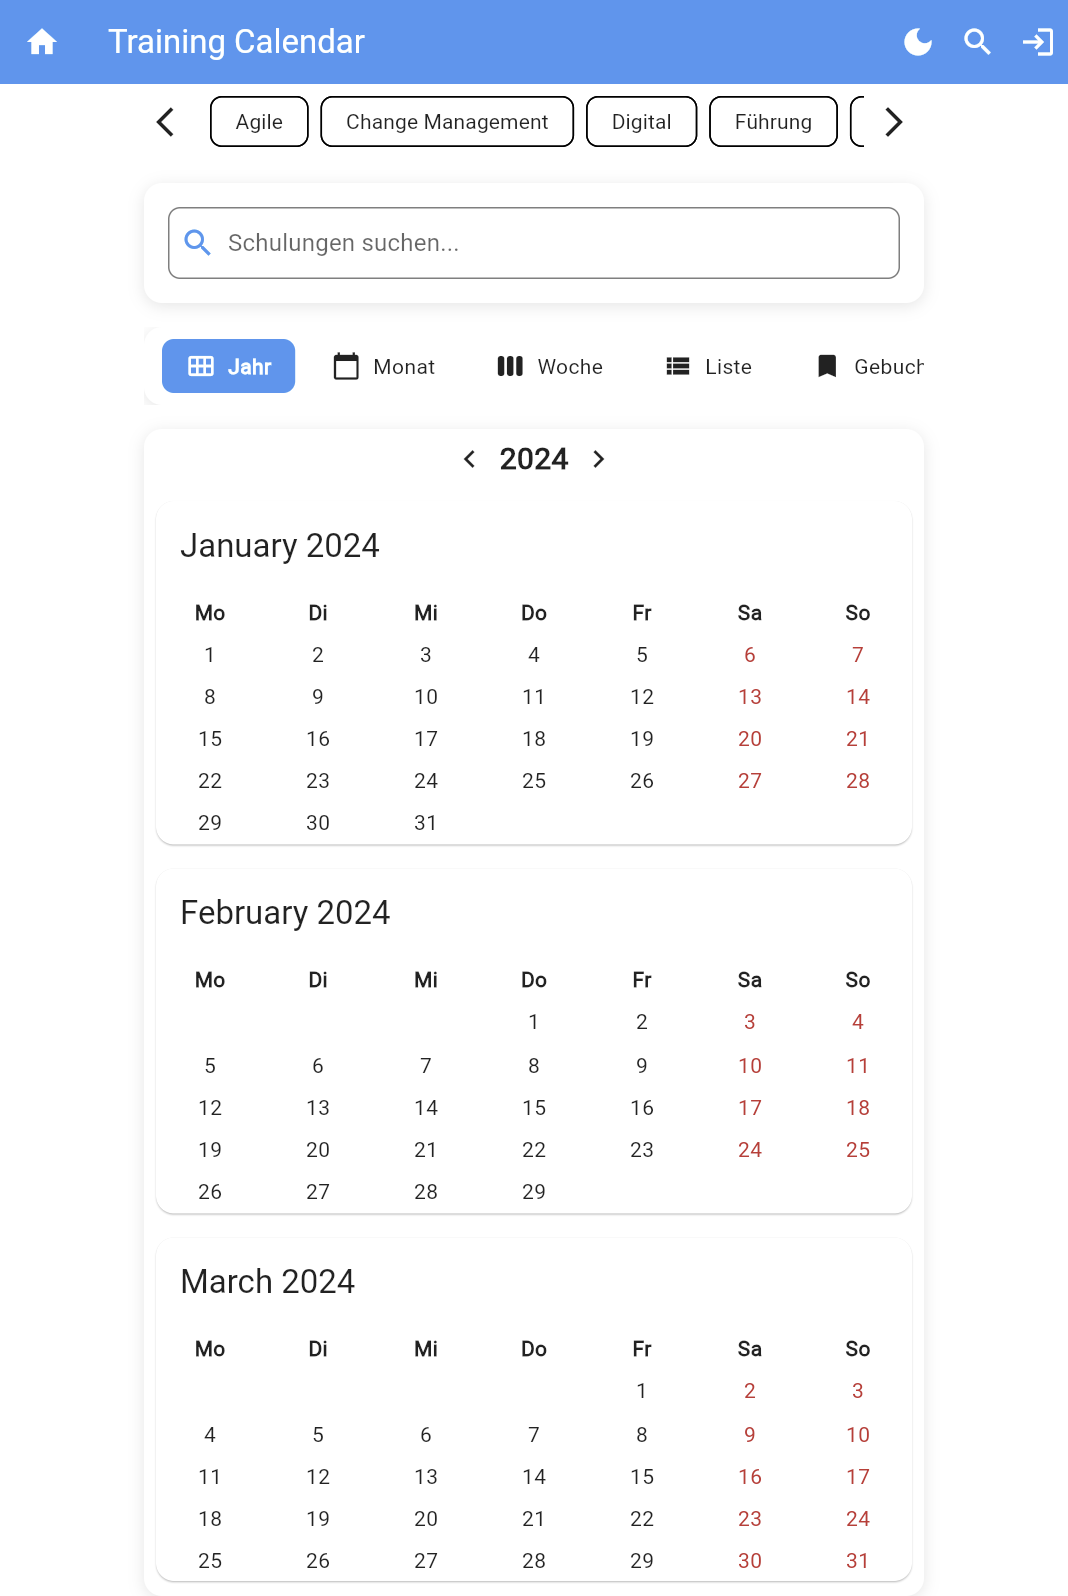
\includegraphics[scale=0.2]{img/flutter_01.png}
        \caption{ Jahresansicht}
        \label{Jahr}
    \end{figure}
  
    \item \textbf{Monatsansicht:} Hier wird der aktuelle Monat detailliert dargestellt (\ref{Monat}). 
Die Monatsansicht zeigt alle Tage eines Monats in einer Rasterdarstellung an, wobei der aktuelle Tag hervorgehoben wird, wie beispielsweise der ------------------ im Screenshot. Mithilfe der Pfeiltasten links und rechts kann man zwischen den Monaten wechseln, um Termine in anderen Zeiträumen zu betrachten.
Der Benutzer kann jeden einzelnen Tag im Monat aufrufen, um mehr Informationen zu den jeweiligen Schulungen zu erhalten.     
\begin{figure}[htbp!]
        \centering
        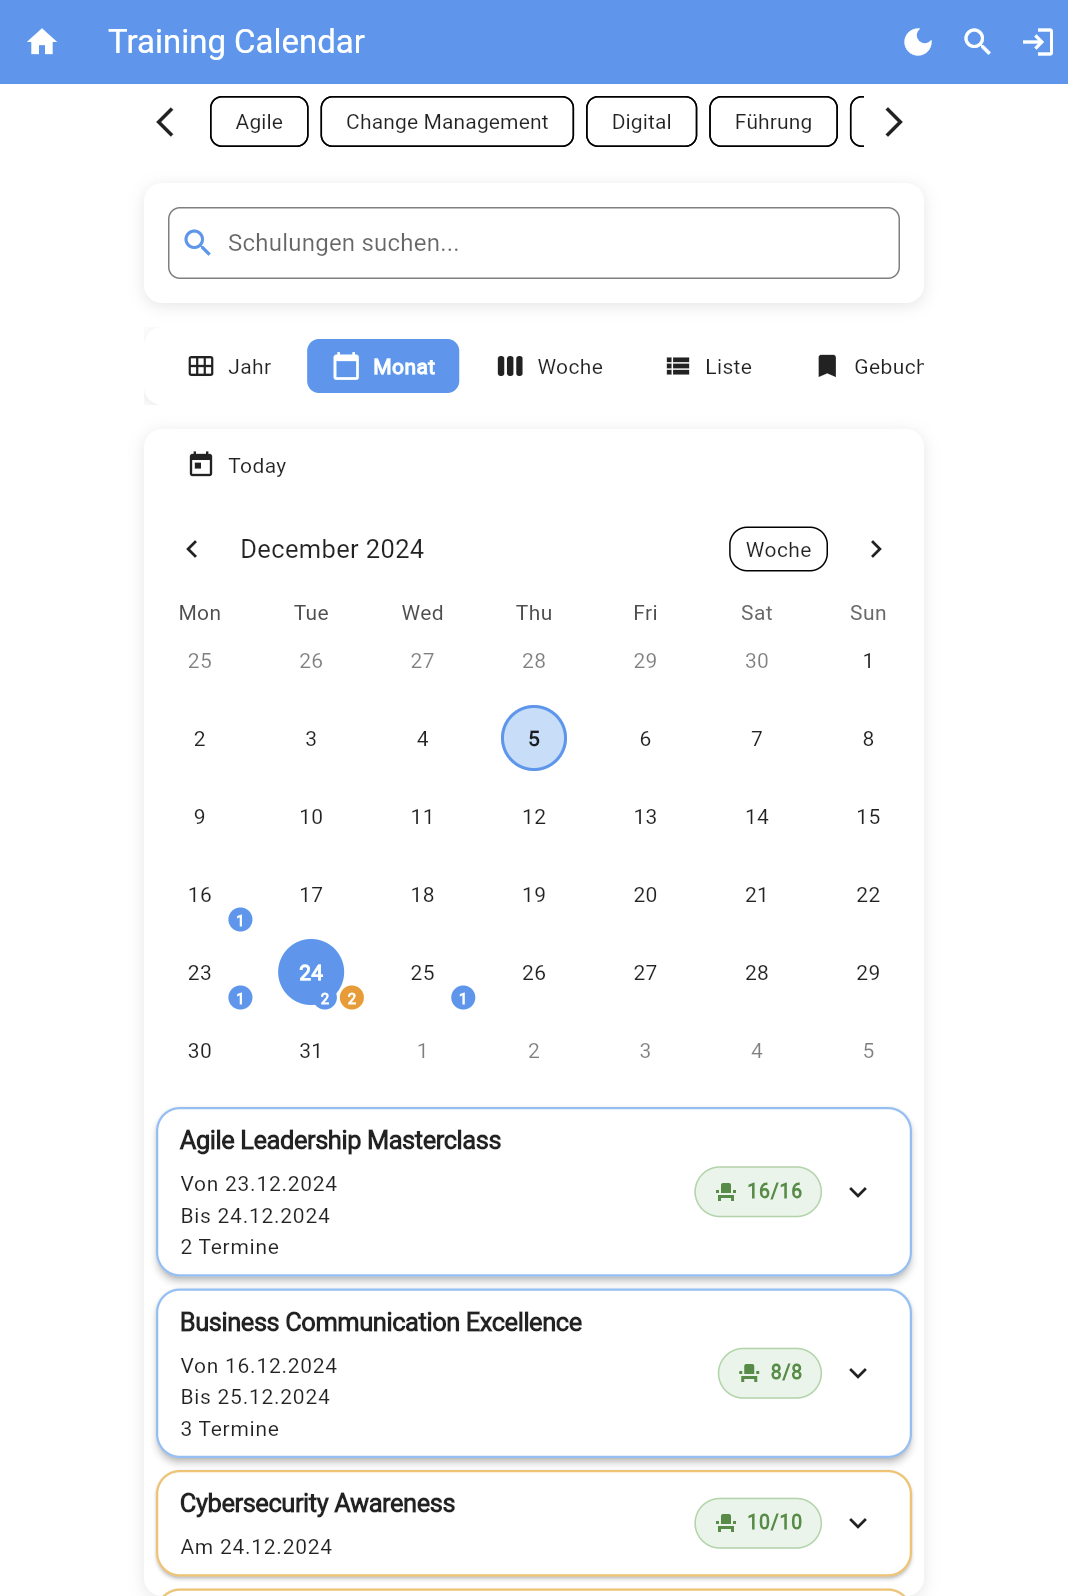
\includegraphics[scale=0.2]{img/flutter_05.png}
        \caption{Monatsansicht}
        \label{Monat}
    \end{figure}

    \item \textbf{Wochenansicht:} In dieser Ansicht (\ref{Woche}) werden die Schulungsdaten in einer Wochenübersicht angezeigt. Dies ist besonders hilfreich, um kurzfristige Schulungen und Termine in der kommenden Woche zu überprüfen und zu verwalten. Der Benutzer hat die Möglichkeit, durch die Wochentage zu blättern und gezielt nach freien Zeiträumen zu suchen.
    \begin{figure}[htbp!]
        \centering
        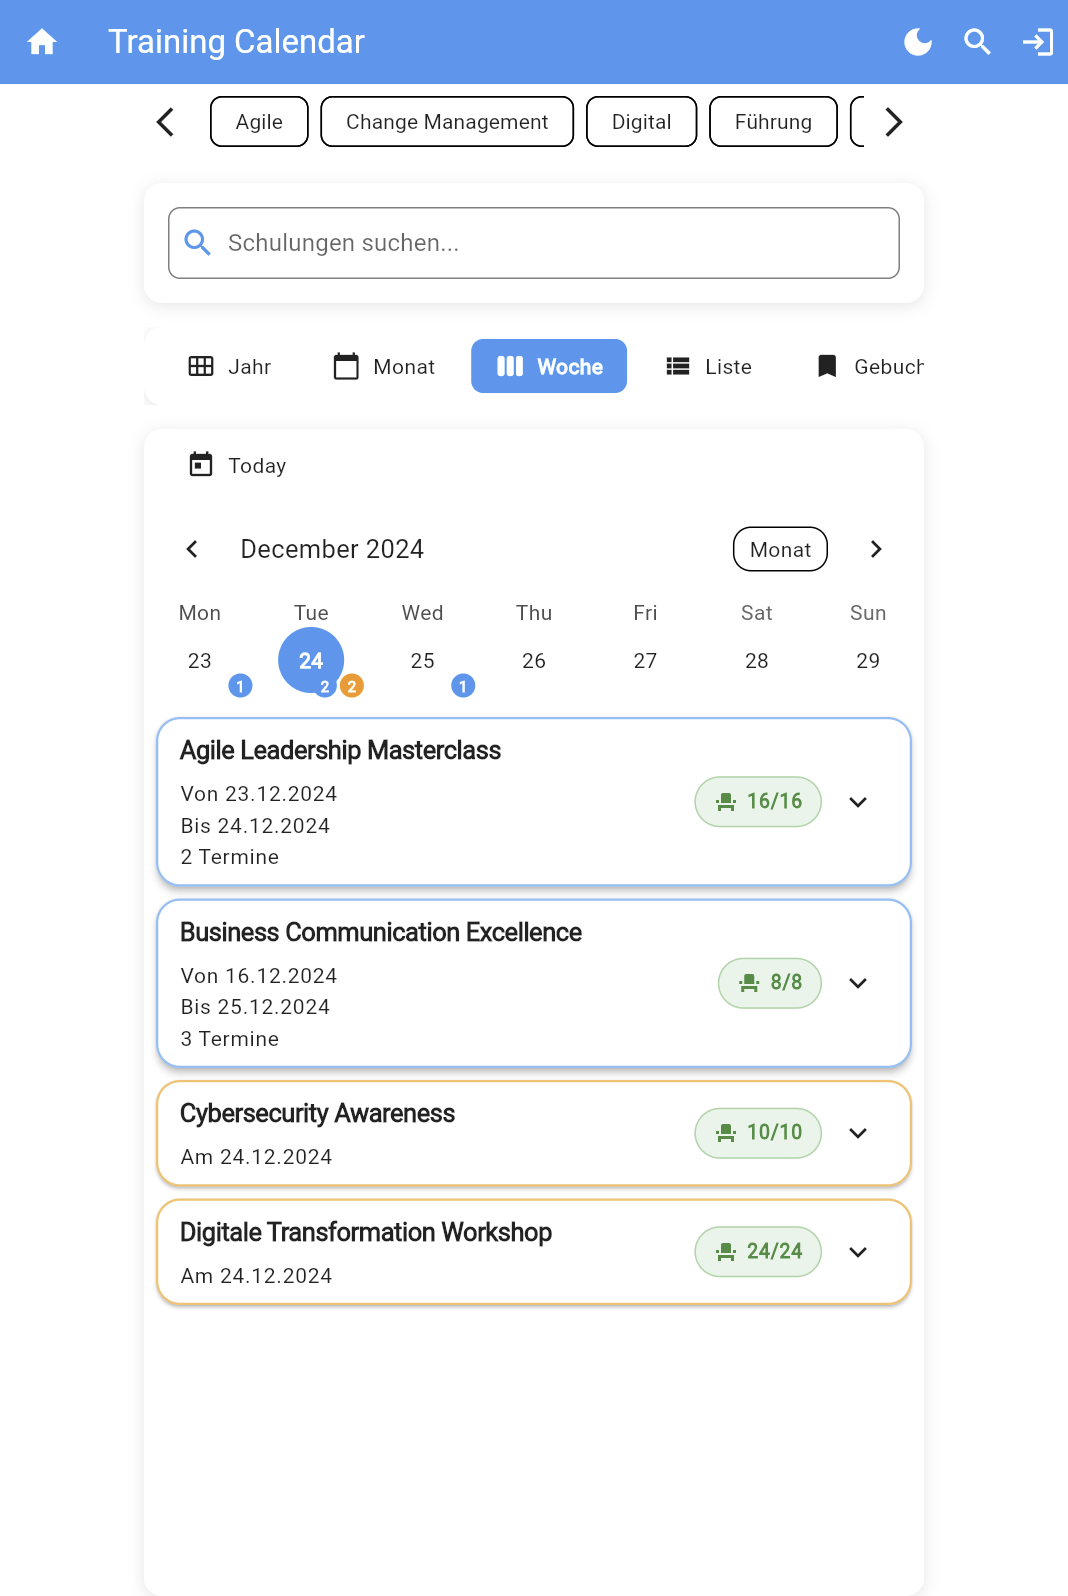
\includegraphics[scale=0.2]{img/flutter_08.png}
        \caption{Wochenansicht}
        \label{Woche}
    \end{figure}

    \item \textbf{Listenansicht:} Alle verfügbaren Schulungen sind in einer übersichtlichen Liste aufgeführt (\ref{List}). Der Benutzer kann durch diese Liste scrollen, um Informationen zu verschiedenen Schulungen wie Titel, Datum, Uhrzeit und Ort zu erhalten. In dieser Ansicht werden auch Sortierfunktionen angeboten, mit denen der Benutzer gezielt nach bestimmten Schulungen suchen kann. Die „Liste“-Ansicht ist besonders hilfreich, um alle Termine in einer scrollbaren Liste darzustellen, was einen schnellen Überblick über anstehende Events ermöglicht.
    \begin{figure}[htbp!]
        \centering
        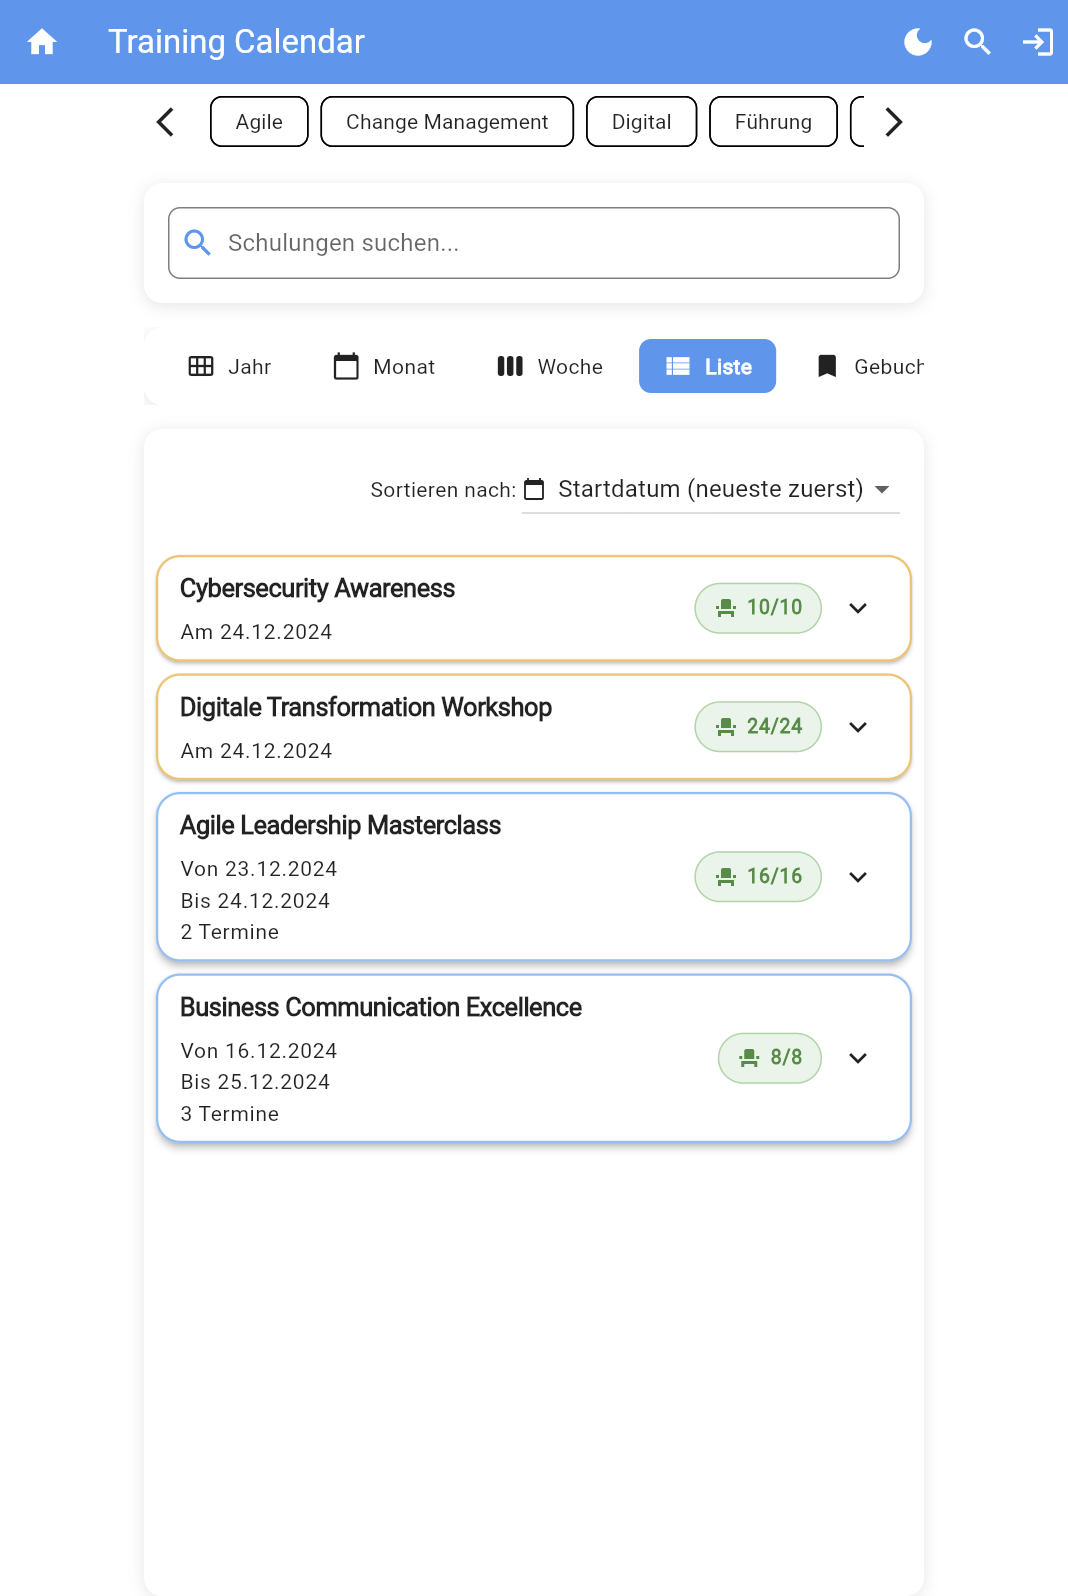
\includegraphics[scale=0.2]{img/flutter_09.png}
        \caption{ Listenansicht }
        \label{List}
    \end{figure}

    \item \textbf{Gebucht-Ansicht:} In der Gebucht-Ansicht (\ref{Gebucht})  werden alle bereits gebuchten Schulungen des Benutzers aufgelistet. Hier kann der Benutzer seine kommenden Termine einsehen, Änderungen vornehmen oder auch Schulungen absagen, falls erforderlich. Diese Ansicht hilft dabei, den Überblick über die eigenen gebuchten Veranstaltungen zu behalten.
\begin{figure}[htbp!]
        \centering
        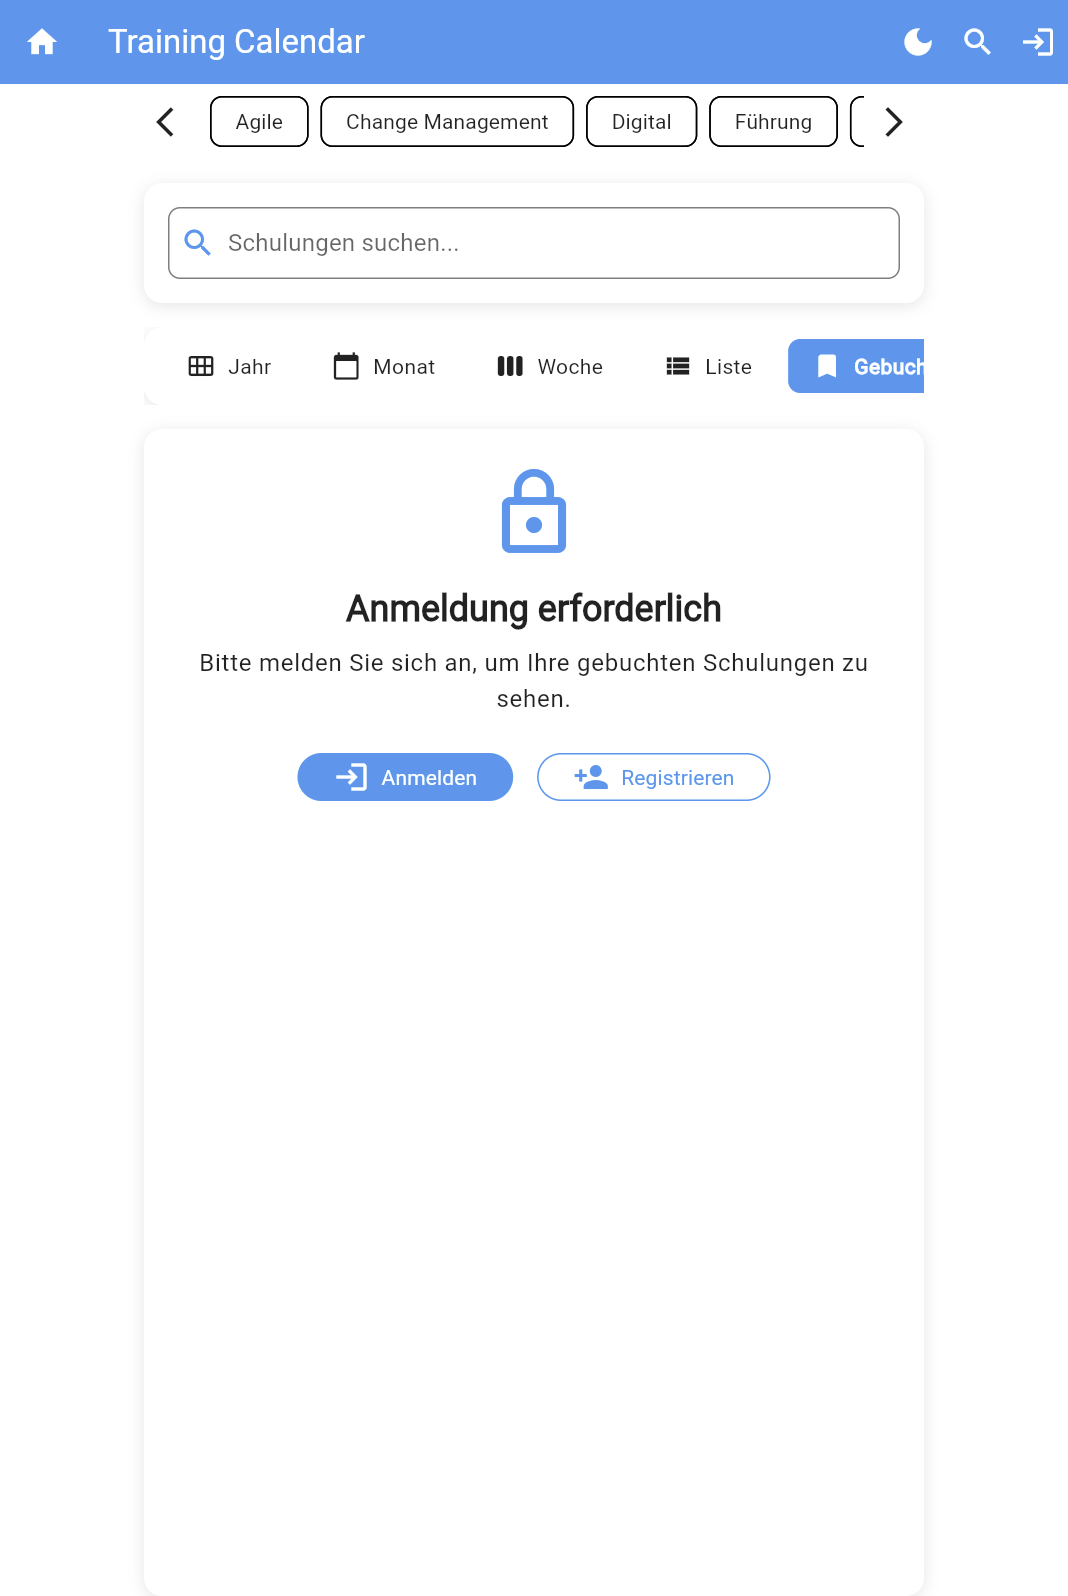
\includegraphics[scale=0.2]{img/flutter_11.png}
        \caption{Gebucht-Ansicht unangemeldet}
        \label{Gebucht}
    \end{figure}
Hier wird einem unangemeldeten Benutzer angezeigt, dass er sich zuerst anmelden muss. So sieht die Ansicht für angemeldete Benutzer aus (\ref{Gebucht2}): 
\begin{figure}[htbp!]
        \centering
        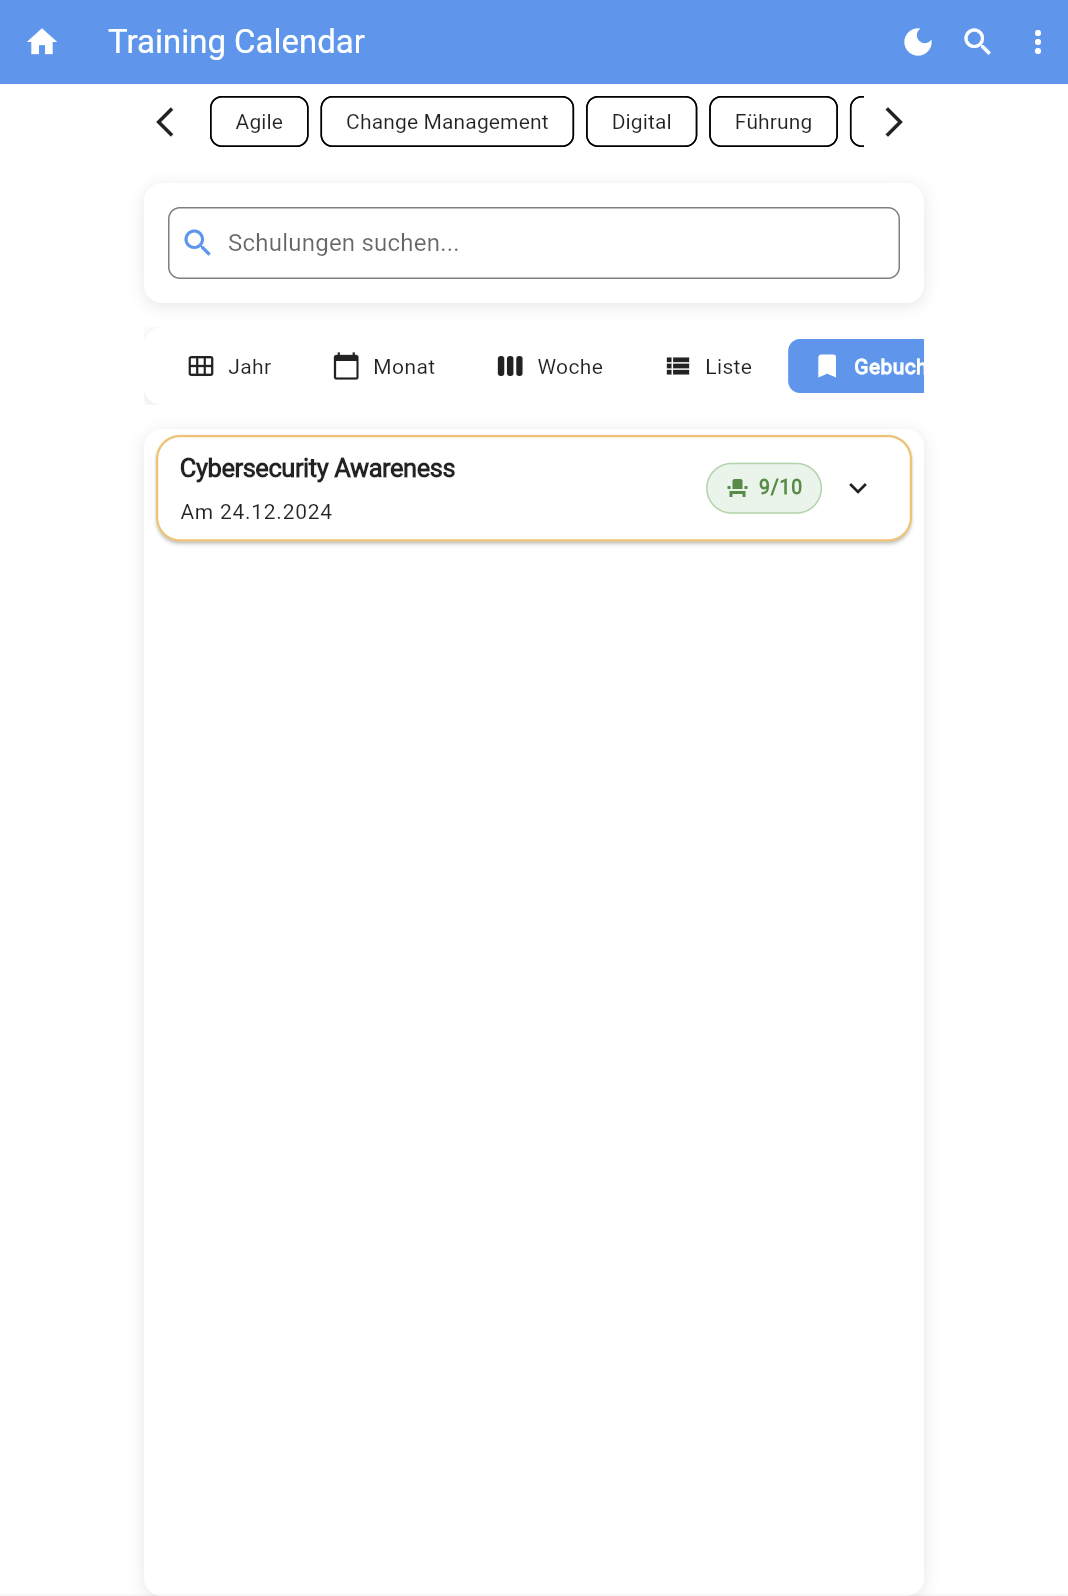
\includegraphics[scale=0.2]{img/flutter_20.png}
        \caption{Gebucht-Ansicht angemeldet}
        \label{Gebucht2}
    \end{figure}
Die Buchungen stehen übersichtlich untereinander aufgelistet. Für eine detailreichere Ansicht kann man Buchungen mit einem Klick aufklappen (\ref{Gebucht3}):
\begin{figure}[htbp!]
        \centering
        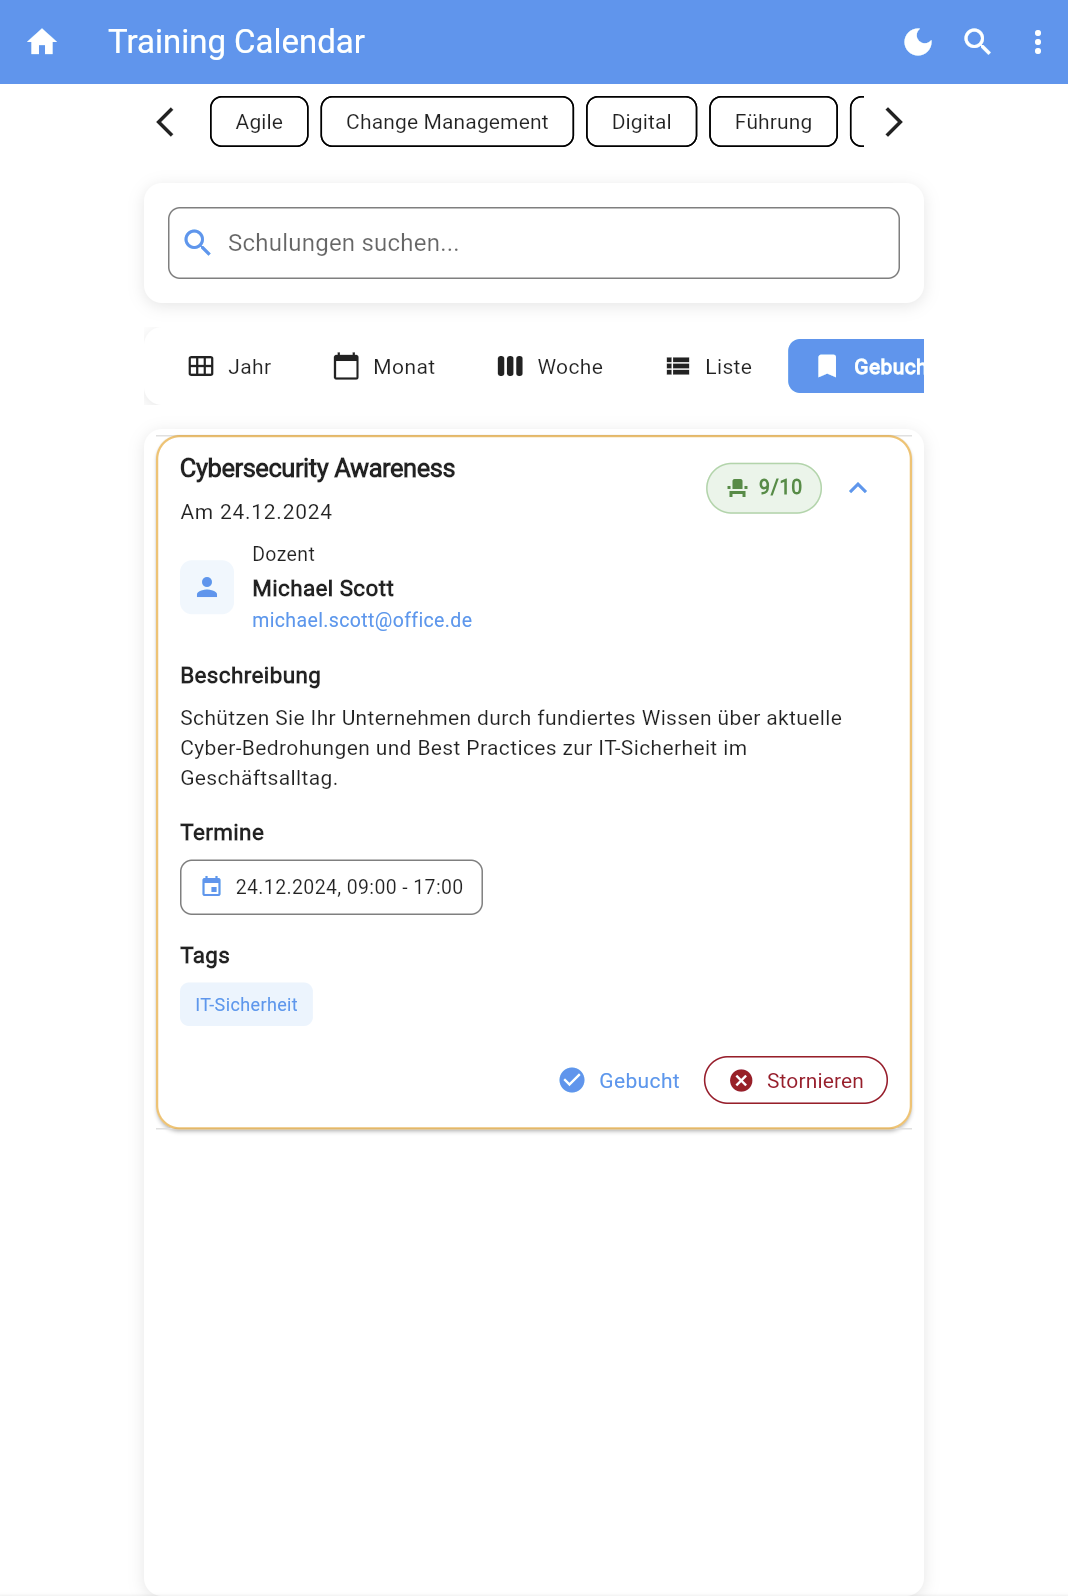
\includegraphics[scale=0.2]{img/flutter_21.png}
        \caption{Gebucht-Ansicht angemeldet ausgeklappt}
        \label{Gebucht3}
    \end{figure}
Der „Gebucht“-Button dient dazu, nur Termine anzuzeigen, die der Benutzer bereits gebucht hat.

\item \textbf{Such-Ansicht:} Weiterhin gibt es eine Suchleiste ganz oben über den Ansichten. Es kann nach einem Termin, einem Schulungsnamen oder einem Dozenten gesucht werden. Oben befindet sich ein Suchfeld, in das Benutzer Stichworte oder Tags eingeben können, um gezielt nach bestimmten Schulungen oder Ereignissen zu suchen. Direkt daneben gibt es die Option, Filter nach Tags anzuwenden, um die Ansicht weiter zu personalisieren.
\begin{figure}[htbp!]
        \centering
        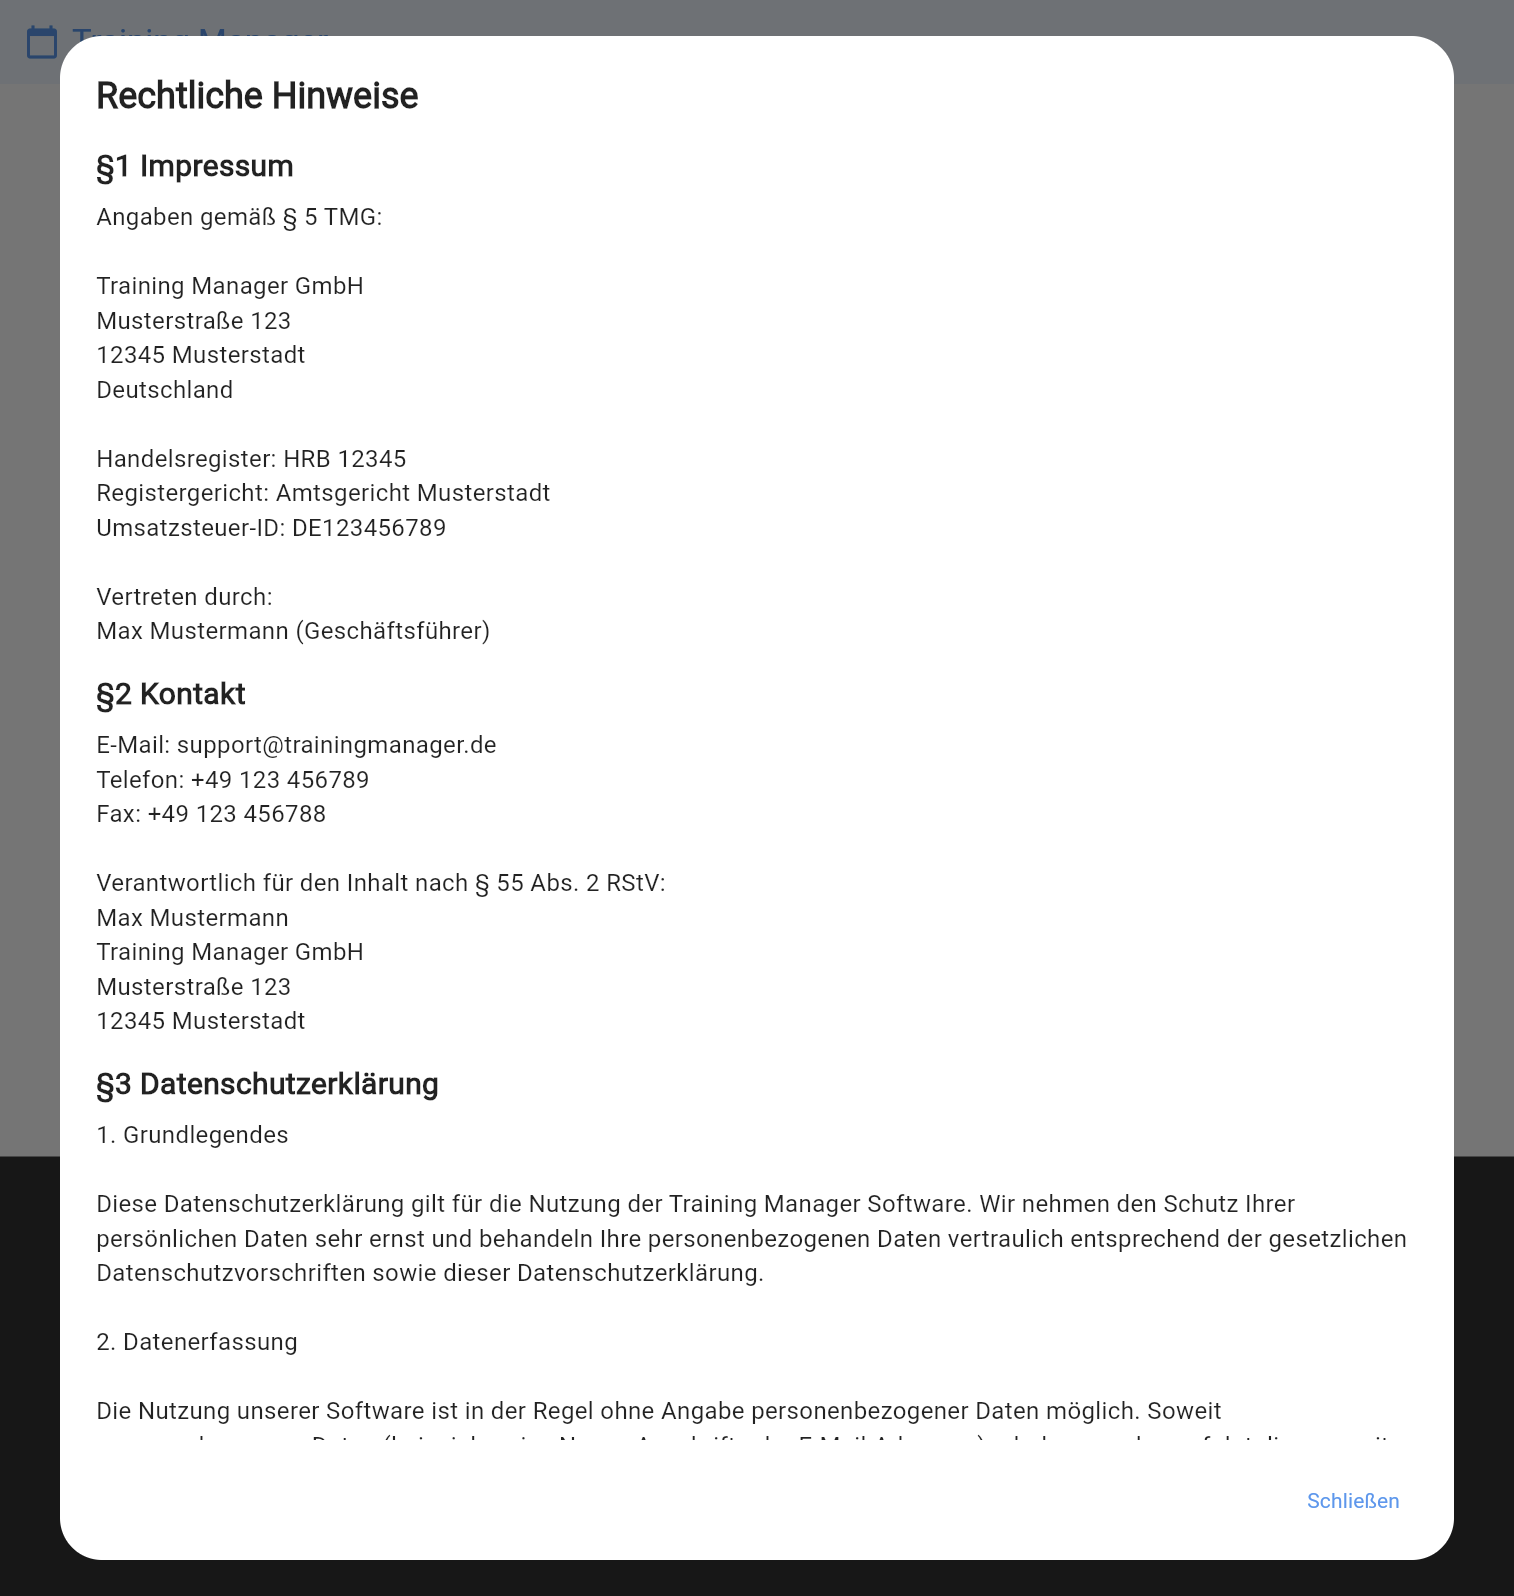
\includegraphics[scale=0.2]{img/flutter_32.png}
        \caption{Such-Ansicht}
        \label{Suche}
    \end{figure}
\end{itemize}

Durch die klare Markierung des aktuellen Tages können Benutzer schnell erkennen, welcher Tag heute ist, ohne die Ansicht manuell zu suchen. 
Zusätzlich kann der Benutzer mit der Nachtmodus-Schaltfläche (oben rechts) die Ansicht zwischen Tag- und Nachtmodus wechseln, was die App auch in dunklen Umgebungen angenehm lesbar macht. 


\begin{figure}[htbp!]
    \centering
    \begin{subfigure}[b]{0.45\textwidth}
        \centering
        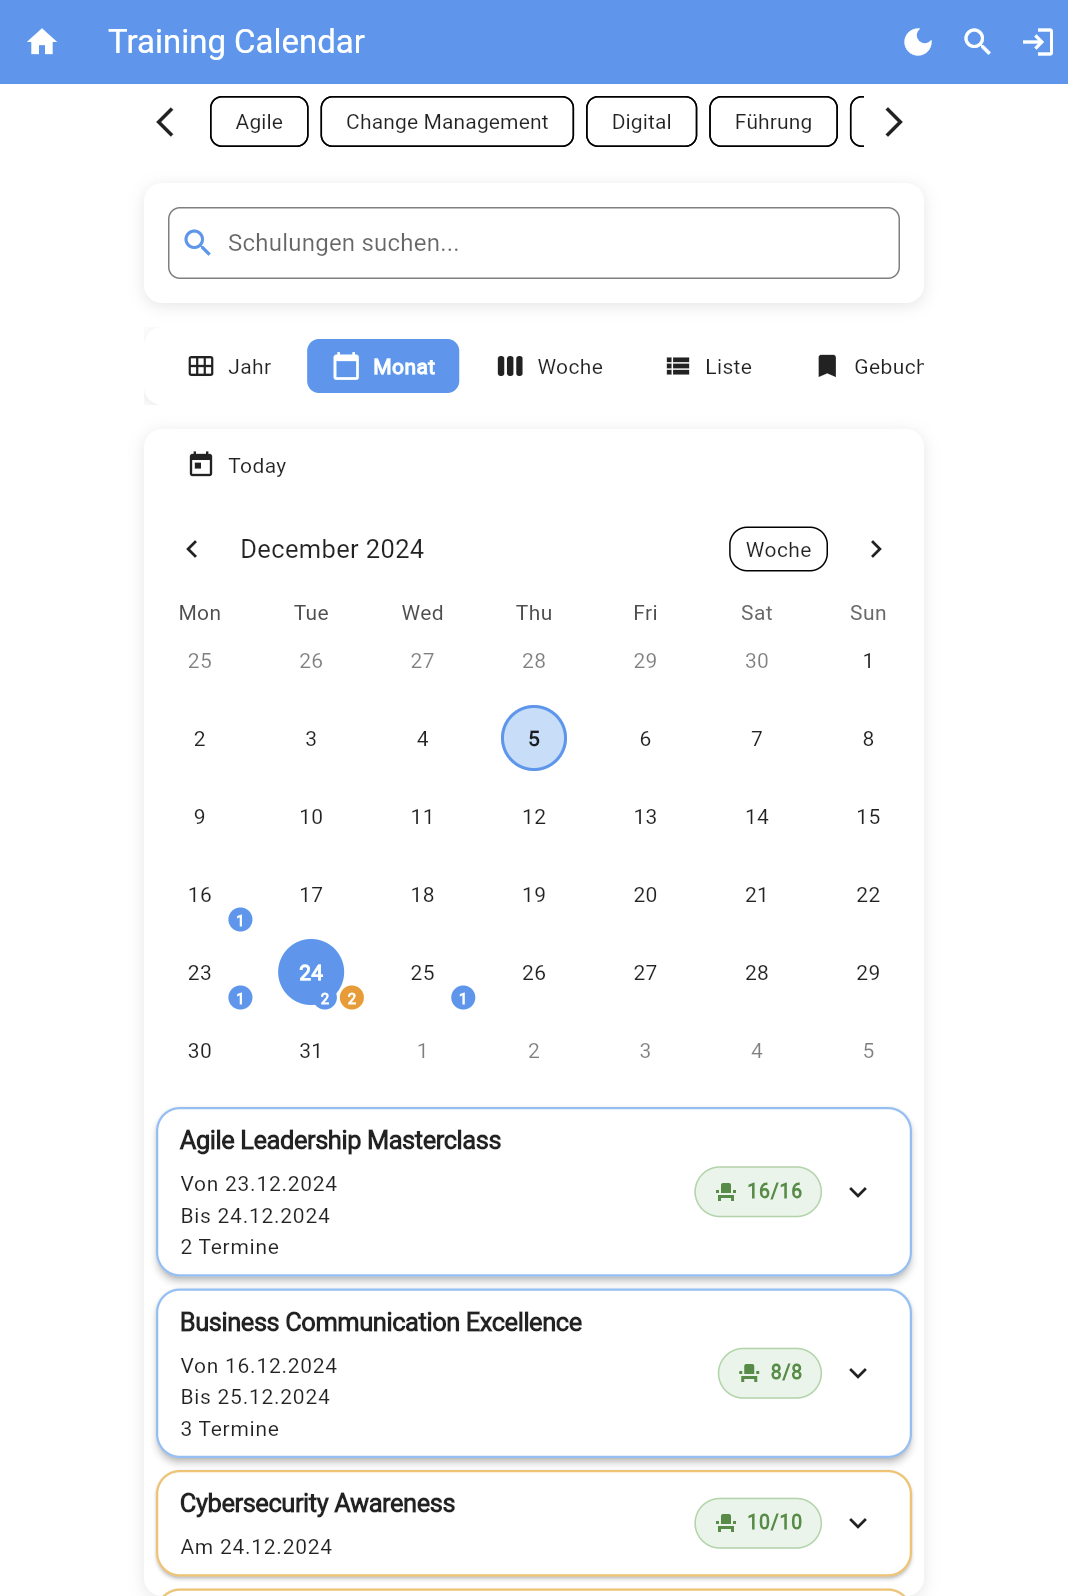
\includegraphics[scale=0.2]{img/flutter_05.png}
        \caption{Normale Ansicht}
        \label{fig:1}
    \end{subfigure}
    \hfill
    \begin{subfigure}[b]{0.45\textwidth}
        \centering
        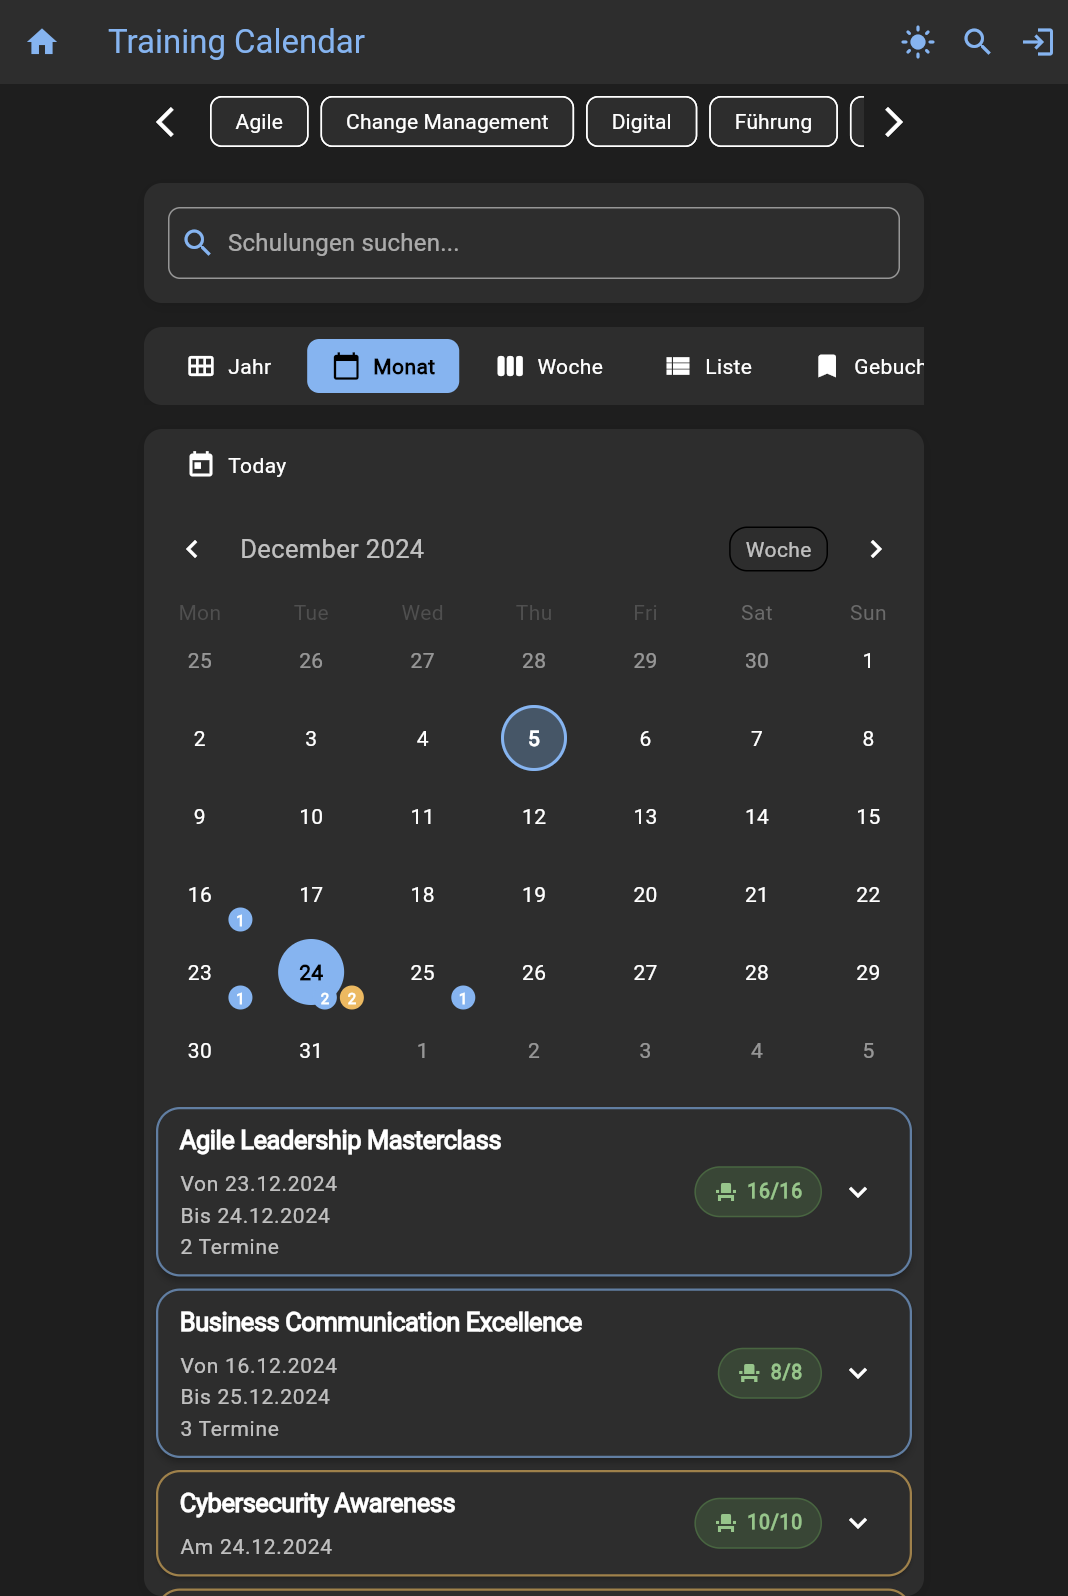
\includegraphics[scale=0.2]{img/flutter_12.png}
        \caption{Ansicht im Dark mode}
        \label{fig:zweitens}
    \end{subfigure}
    \caption{ Ansicht im Dark mode}
    \label{fig:2}
\end{figure}

Eine kleine Home-Schaltfläche in der oberen linken Ecke führt jederzeit zurück zur Startseite. 
Die App ist darauf ausgelegt, schnell und effizient zwischen verschiedenen Ansichten zu wechseln und die gesuchten Informationen mit wenigen Klicks zugänglich zu machen. Die Markierungen der Schaltflächen und das Design der Kalenderansicht sind minimalistisch und lenken nicht vom Wesentlichen ab. Durch die Kombination von Suchfunktionen und personalisierbaren Ansichten wird die Nutzung besonders benutzerfreundlich gestaltet.

%Anmeldung noch beschreiben.!!!!!!!!!!!!!!!!!!!!!!!!!!!!!!!!!!!
